\section{Motivation}
\label{sec:motivation}

Figure~\ref{fig:motivation} shows a short snapshot of how the
frequency of the \Cpu adapts to four input events for two different
\Dvfs governors. WOW so motivating.

%% FIGURE: Workload Snapshot -------------------------------------------------
\begin{figure}[t!]
  \begin{centering}
    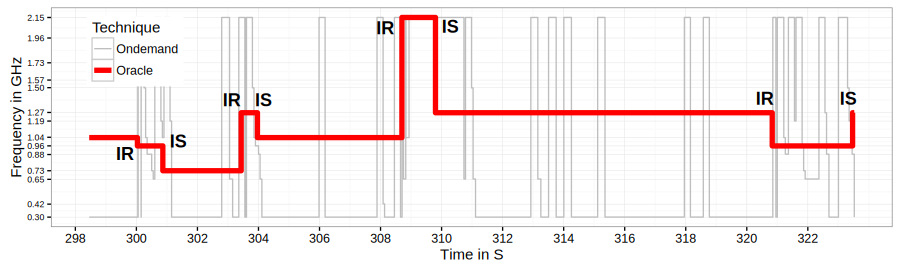
\includegraphics[width=1\columnwidth]{figures/motivation}
    \par
  \end{centering}
  \caption{Snapshot of the behavior of the \Ondemand governor and
	  another more energy efficient governor for one of this study's
	  interactive workloads. \textbf{IR} indicates when user input was
	  received and \textbf{IS} indicates the earliest time when the user
	  would perceive the input as serviced.
  \label{fig:motivation}}
\end{figure}
% ------------------------------------------------------------------------------

